\documentclass[12pt]{article}

\usepackage{amsfonts}
\usepackage[english]{babel}
\usepackage[a4paper, total={14cm, 26cm}]{geometry}
\usepackage{graphicx}
\usepackage{listings}
\usepackage{multicol}
\usepackage{tabularx}
\usepackage{xcolor}

\definecolor{codegreen}{rgb}{0,0.6,0}
\definecolor{codegray}{rgb}{0.5,0.5,0.5}
\definecolor{codepurple}{rgb}{0.58,0,0.82}
\definecolor{backcolour}{rgb}{0.95,0.95,0.92}

\lstdefinestyle{mystyle}{
    backgroundcolor=\color{backcolour},
    commentstyle=\color{codegreen},
    keywordstyle=\color{magenta},
    numberstyle=\tiny\color{codegray},
    stringstyle=\color{codepurple},
    basicstyle=\ttfamily\footnotesize,
    breakatwhitespace=false,
    breaklines=true,
    captionpos=b,
    keepspaces=true,
    numbers=left,
    numbersep=5pt,
    showspaces=false,
    showstringspaces=false,
    showtabs=false,
    tabsize=2
}

\lstset{style=mystyle}

% Prefix
\title{Real-time Speech Recognition and Speaker Diarization: Toward Inclusive University Lectures}
\author{Jannik Schmied}
\date{\today}

% Start: Document
\begin{document}

\maketitle

% Abstract
\textbf{\abstractname}
This paper presents a comprehensive exploration into the realm of real-time speech recognition coupled with speaker diarization to amplify accessibility in university lecture settings, specifically catering to the deaf community. Several methodologies were analyzed, ranging from Convolution Neural Networks (CNNs) operating on audio datasets to state-of-the-art frameworks offered by entities like NVIDIA. However, the principal challenge remained harmonizing speech recognition with speaker diarization. Two primary strategies emerged as the most viable: a hybrid approach leveraging OpenAI's Whisper for transcription, and an online method anchored in AssemblyAI. Both pathways were underpinned by diverse advantages and challenges. While Whisper's multilingual capacities offered versatility, the online route, although English-centric, circumvented hardware constraints. The hybrid solution’s efficacy in real-time transcription and speaker shifts was gauged against AssemblyAI's model, revealing distinct use cases for each based on situational requirements. Current implementations, potential improvements, and integration into user-friendly interfaces such as Streamlit were also discussed. An area for subsequent research lies in the technology's acceptance among its target demographic, especially when juxtaposed with native sign language interpreters. Through this exploration, we endeavor to make academic settings more inclusive, fostering seamless communication for all attendees.

\section{Motivation}
\label{sec:motivation}

In the age of digital learning, the need to make education accessible to all cannot be overemphasized. University lectures, serving as a cornerstone of advanced education, present valuable content that must be universally accessible, irrespective of auditory challenges. While transcription services provide a textual alternative to spoken words, merely converting speech to text fails to capture the full dynamics of a classroom, especially when multiple speakers, each with distinct insights, are involved. Real-time speech recognition with speaker diarization steps in to bridge this gap, offering not only the advantage of instant transcription but also an insight into speaker changes, providing an essential context. For individuals with hearing impairments, such advancements can mean the difference between a fragmented understanding and a comprehensive grasp of lecture content. By exploring and refining these technologies, we move closer to an inclusive learning environment where auditory barriers are diminished.

\section{Concept}
\label{sec:concept}

The pivotal challenge lay in the integration of two distinct approaches: speech recognition and speaker diarization. Throughout the research process, several potential methodologies emerged, warranting deeper exploration.

\subsection{Self-trained Neural Networks}
\label{ssec:cnn}

Initially, a Convolutional Neural Network (CNN) was employed to detect speaker changes. The input features for this model were derived from audio data transformed into Mel-Spectrograms or Fast Fourier Transformed (FFT) representations. To train the model, the Audio MNIST dataset \cite{AudioMNIST} was utilized, which is a popular choice for audio-based tasks due to its diverse audio samples. Despite several training epochs and rigorous optimization attempts, this approach only yielded an average accuracy of 0.84. This performance was suboptimal and fell short of the anticipated results. Alternative techniques, such as employing Feed-Forward Neural Networks or Recurrent Neural Networks—also cited in the literature—might enhance outcomes. However, after the experiments conducted, these were deemed beyond the scope, leading the focus towards other strategies. \cite{Jia2021}

\subsection{NVIDIA NeMo}
\label{ssec:nemo}

A potential remedy for the challenges previously encountered lies in employing a pretrained model tailored for speaker diarization. NVIDIA offers such a model within their NeMo framework. As of this writing, NeMo is in a beta phase, and its documentation remains somewhat preliminary. Furthermore, its exclusive compatibility with NVIDIA GPUs restricts its versatility, potentially limiting the subsequent software's deployment across a diverse range of devices.

\subsection{AssemblyAI}
\label{ssec:aai}

Addressing the challenge of ensuring software operability across diverse devices without relying on robust hardware components, an API-centric approach emerges as a solution. This method substantially alleviates the majority of hardware prerequisites, requiring only a stable internet connection from the user's end. However, it also introduces a dependency on consistent online connectivity.

\subsection{Whisper and PyAnnote}
\label{ssec:whisper}

In our exploration, we delved into a hybrid methodology, leveraging OpenAI's Whisper for speech-to-text transcription, paired with PyAnnote and its pretrained speaker diarization model \cite{Bredin2019}. Within this setup, speech recognition is primarily GPU-dependent, while diarization processes are delegated to the Hugging Face's API resources. For situations lacking a sufficiently powerful GPU, Whisper offers a cloud-based solution through OpenAI's API, providing a pathway to transition the approach to an entirely online system. Additionally, for those prioritizing offline functionalities, the Huggingface model is available for download, eliminating the need for persistent network connectivity.

\subsection{Comparision and Decision}
\label{ssec:comp}

% Comparison table
\begin{table}[h]
    \centering
    \begin{tabular}{|l|c|c|c|}
        \hline
        \textbf{Approach} & \textbf{Offline?} & \textbf{GPU neccessary?} & \textbf{Training necessary?} \\ 
        \hline
        CNN Mel-Spec & Yes & Yes & Yes \\ 
        \hline
        CNN FFT & Yes & Yes & Yes \\ 
        \hline
        NVIDIA NeMo & Yes & Yes & Only fine tuning \\ 
        \hline
        AssemblyAI & No & No & No \\ 
        \hline
        Whisper + PyAnnote & Yes & Only for offline use & No \\ 
        \hline
    \end{tabular}
    \caption{Technology comparison} 
    \label{tab:tech-comp}
\end{table}

\noindent Given the limitations of both the self-trained CNNs and NVIDIA's NeMo as outlined earlier, two viable Proofs of Concept emerge for implementation: the online solution via AssemblyAI, and the hybrid method that integrates Whisper with PyAnnote.

\section{Implementation}
\label{sec:implementation}

The approaches pinpointed were subsequently developed into functional Proofs of Concept (PoCs). Both PoCs were crafted in Python, utilizing a blend of native and third-party libraries. A comprehensive list of these libraries is accessible in the project's Git repository.

\subsection{Online Approach: AssemblyAI}
\label{ssec:online}

\subsubsection{Speech-to-text and speaker diarization}

Both tasks, the speech-to-text operation as well as speaker diarization are performed using the AssemblyAI API.

AssemblyAI offers a websocket-based API endpoint for its real-time transcription model. To utilize this, an asynchronous connection is initiated allowing for the continuous streaming of data from the microphone's audio feed to the API to realize audio transcription.

Conversely, the diarization process is executed through AssemblyAI's Python SDK, which processes the recent audio stream data. Subsequent to processing, the results are collated and presented to the user.

\subsubsection{GUI: Streamlit}

Streamlit is an open-source Python library that makes it easy to create and share custom web apps for machine learning and data science. For visualization, Streamlit is employed, ensuring the results are showcased in an intuitive manner for viewers.  

\subsubsection{Final Remarks}

One limitation of this method lies in its cost; the API usage typically incurs an expense of about 1 USD for a standard lecture's duration. However, there's optimism that these costs will reduce in the future. Additionally, a current constraint is the model's exclusive compatibility with English inputs.

In terms of data analysis, the API assists the user in form of a variety of metadata that is included in the Response, for example, the confidence for both the entire transcription as well as every individual word.

\subsection{Hybrid Approach: Whisper and PyAnnote}
\label{ssec:offline}

\subsubsection{Speech-to-text: Whisper}

In a manner analogous to the previously outlined online method, this approach draws from the microphone's audio stream. The distinction lies in its subsequent processing, which is entrusted to OpenAI's Whisper. Initially, the latest audio segment is captured and stored in a temporary file, which then undergoes transcription. In a parallel process, the SpeechRecognition library is leveraged to execute several additional tasks, including Voice Activation Detection (VAD), Pause Detection, and Phrase Completion Detection.

\subsubsection{Speaker diarization: PyAnnote}

Upon completion of the transcription phase, the process advances to diarization. This step leverages the PyAnnote library in conjunction with a pretrained model sourced from Huggingface. Notably, this stage posed the most formidable challenge, necessitating a delicate balance between accuracy and computational performance. Relying solely on the latest audio snippet introduced the potential pitfall of overlooking speaker transitions. As a remedy, a secondary temporary file—encompassing the last $n$ snippets—was formulated and routinely updated. This augmented file then informs the diarization function, with its outcomes harmonized with the transcriptions. The synthesized results, linked with the relevant timestamp, are subsequently relayed to the audience. To pinpoint the optimal value for $n$, an extensive battery of tests was conducted and the findings meticulously dissected.

\begin{figure}[h]
    \centering
    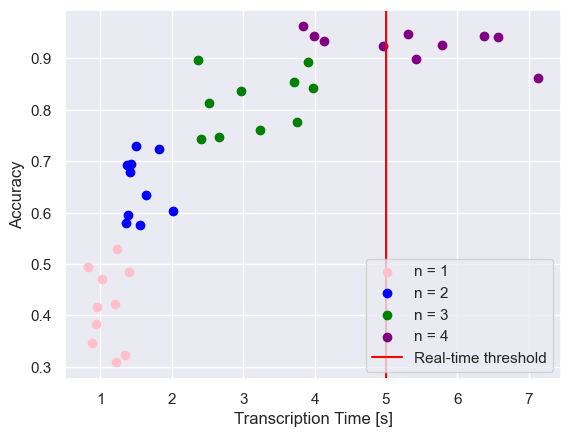
\includegraphics[width=0.8\linewidth]{time-accuracy-plot.png}
    \caption{Test results} 
    \label{fig:test-results} 
\end{figure}

From the array of tests conducted, $n = 3$ emerged as the optimal choice, satisfying the hypothesis test criteria with $P > 0.95$ while concurrently ensuring that the total processing duration remained under the self-imposed threshold of 5 seconds.

\subsubsection{Offline Mode}

This methodology supports complete offline functionality. Consequently, the diarization model needs to be pre-downloaded, and its loading input replaced with the local model path. Nonetheless, this introduces elevated hardware demands. Tests conducted indicate that, at a minimum, an NVIDIA 3000 Series GPU equipped with 8 GB of VRAM is requisite for efficient operation.

\subsubsection{Online Mode}

To circumvent the aforementioned hardware constraints, an alternative lies in leveraging OpenAI's API for audio transcription. Unlike AssemblyAI, OpenAI's documentation doesn't explicitly highlight real-time applications, and the feasibility of such an approach warrants further investigation.

\subsubsection{Final Remarks}

Unlike AssemblyAI's model, Whisper boasts multilingual capabilities, rendering it more versatile for current applications.

Currently, the hybrid approach lacks a dedicated GUI, rendering its output exclusive to the Terminal. To remedy this limitation, Streamlit stands as a straightforward solution, mirroring its application elsewhere. Alternatively, integration with presentation software, such as PowerPoint, offers another potential avenue for enhancement.

\section{Conclusion and Outlook}
\label{sec:conclusion}

% Trade-off accuracy-performance
Each of the final strategies exhibits its unique advantages and challenges. Consequently, the selection between them hinges on a variety of considerations. When hardware constraints aren't an impediment, the hybrid or entirely offline method might emerge as the preferable option, particularly if language specifications are a concern. Conversely, if hardware presents a limitation, the online strategy anchored in AssemblyAI distinctly excels in English contexts over the hybrid variant. For non-English endeavors, the online modality incorporating Whisper remains a viable choice, though its real-time adaptability warrants further examination.

A pivotal avenue for subsequent research lies in gauging acceptance within the target demographic. Key areas of exploration include the overall receptiveness to the technology and its efficacy in comparison to a native sign language interpreter, the latter being perceived as the gold standard in communicative accessibility.

% Bibliography
\newpage

\nocite{*}

\bibliographystyle{ieeetr}
\bibliography{sources}

\end{document}
